\cleardoublepage
\chapter{Experiment Setup}\label{sec:setup}

\section{Introduction}

The experiment setup consists of several existing components, like a robot system with its gripper, an event-based camera and a computer. However, to fix the event-based camera to the robot and gripper, a mount is needed, which has been designed according to our needs. Moreover, all these components are put together in a certain environment and using a certain software. Finally, due to the changes in the robot system (the addition of the mount and the camera) some adjustments have been made.

\section{Components}
\subsection{Robot system}

The robot system is composed by the robotic arm and controller, named Panda system, or simply Panda, which is a cobot developed and produced by the company Franka Emika GmbH.\\

The robotic arm has 7 DoF, where each axis is actuated through brushless DC motors, which are well-known for their high efficiency, high speed and no maintenance. In ~\Cref{fig:pandarobot} the axes of the arm are depicted as well as the work envelop of it.\\

\begin{figure}[h]
    \centering
    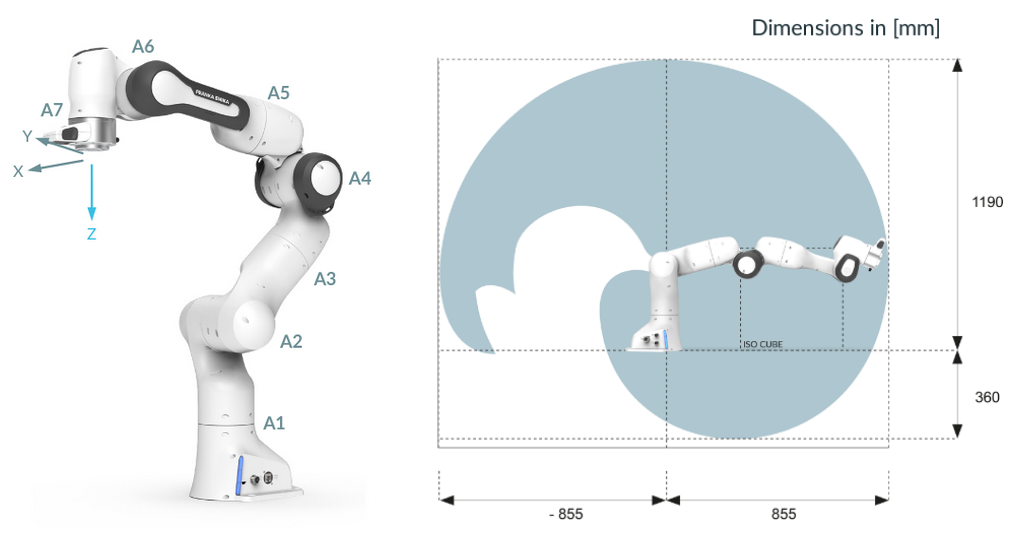
\includegraphics[width=\textwidth]{resources/images/pandarobot}
    \caption{Axes of the Panda robotic arm (left) and its work envelope (right) ~\cite{panda}.}\label{fig:pandarobot}
\end{figure}

The controller refers to the main control computer which is connected to the robotic arm and offers an Ethernet connection for a PC workstation. Additionally, the Panda system includes an emergency stop device integrated between the electricity connection and the controller. This device also enables the guiding mode, which consists of moving the robotic arm manually.

\subsection{Gripper}

The end-effector used for the pick-and-place operation is an electrical two-finger parallel gripper, shown in ~\Cref{fig:pandagripper}. This gripper is specifically designed for Panda, as it communicates directly via the connection in the robotic arm and is also supplied with power from it.

\begin{figure}[h]
    \centering
    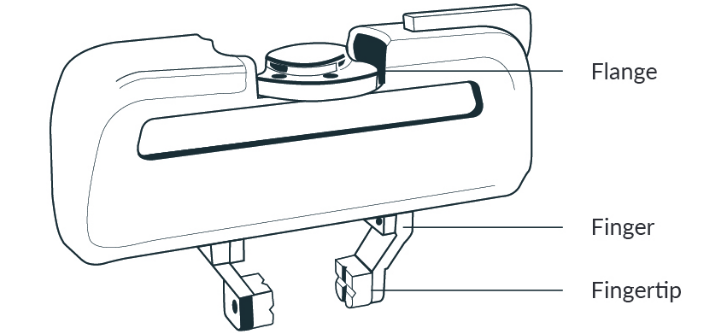
\includegraphics[width=0.6\textwidth]{resources/images/pandagripper}
    \caption{Two-finger parallel gripper ~\cite{panda}.}\label{fig:pandagripper}
\end{figure}

\subsection{Event-based camera}

The used event-based camera is the DAVIS 346, from iniVation, which provides as output not only the events, but also the grayscale frames. We use this camera with its lens, as shown in ~\Cref{fig:davis}.

\begin{figure}[H]
    \centering
    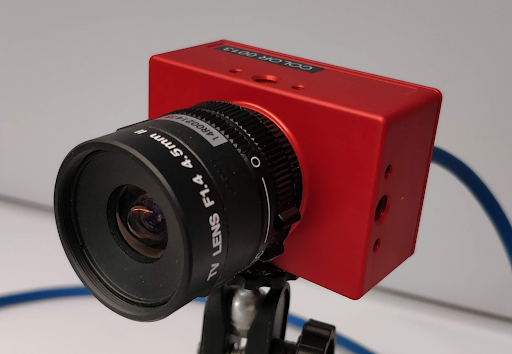
\includegraphics[width=0.4\textwidth]{resources/images/davis}
    \caption{DAVIS 346 event-based camera from iniVation.}\label{fig:davis}
\end{figure}

The DAVIS 346 ~\cite{davis} has a resolution of 346 x 260 pixels, for both events and frames. In terms of the event output, the dynamic range is 120 dB and the latency is 20 $\mu$s. On the contrary, the grayscale dynamic range is 56.7 dB and the maximum frame rate is 40 fps.

\subsection{Computer}

Finally, a computer is needed to connect to the control of the Panda via Ethernet and send commands to the robotic arm and also to connect the event-based camera and process its output.

\section{Design of the camera mount}

In order to assemble the event-based camera to the robotic arm and the gripper we need a camera mount, which has to be designed to make sure the camera has a wide view of the contact between the gripper and the object, such as in the works ~\cite{gelsight2018} and ~\cite{rss2020}. Moreover, this mount should be robust enough to hold the camera firmly, but at the same time being as lightweight as possible. Also, it should provide flexibility in order to be able to adjust the camera's position during the research phase, without having to build a new mount each time.\\

The mount consists of two parts: part A and part B, as shown in ~\Cref{fig:mount}. To design part A, firstly, the connection to the robotic arm and gripper should be considered. Actually, the mount can be fixed with a screw directly to the robotic arm, in the same way as the gripper is fixed. Moreover, in order to reduce vibrations during the movement of the robot, the mount follows the shape of the gripper, thus, providing more stability. Then, an extension is designed with an inclination, such that, once mounted, the camera points towards the gripper. Finally, note that some holes have been introduced to part A with the only aim of reducing the weight of it. In terms of part B, it attaches to DAVIS 346 and to the part A with some screws, providing flexibility when it comes to choose the distance at which the camera is placed. Concretely, the connections of the camera and part B to part A, can be regulated, such that the distance from the gripper's center to the lens (distance \textit{d} indicated in ~\Cref{fig:assembly}) ranges from 10.5 to 19.5 cm, having in total 7 positions separated by 1.5 cm.

\begin{figure}[H]
    \centering
    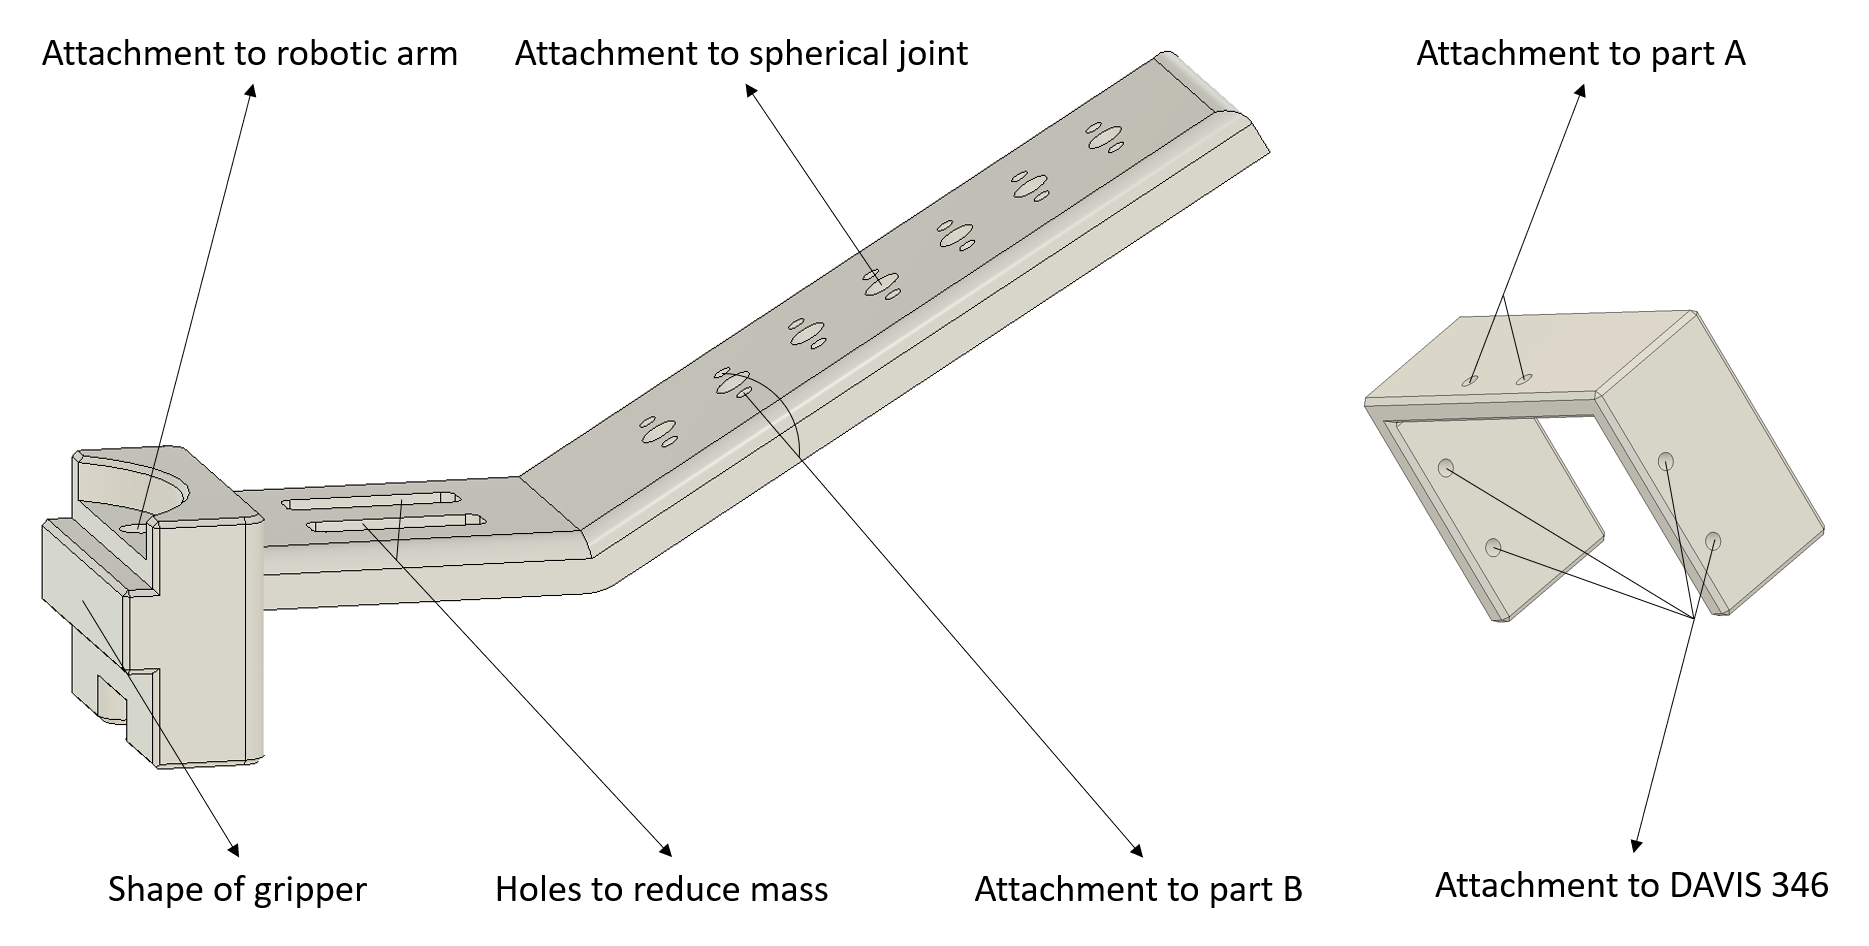
\includegraphics[width=\textwidth]{resources/images/mount_description}
    \caption{Description of the mount: part A (left) and part B (right).}\label{fig:mount}
\end{figure}

\begin{figure}[H]
    \centering
    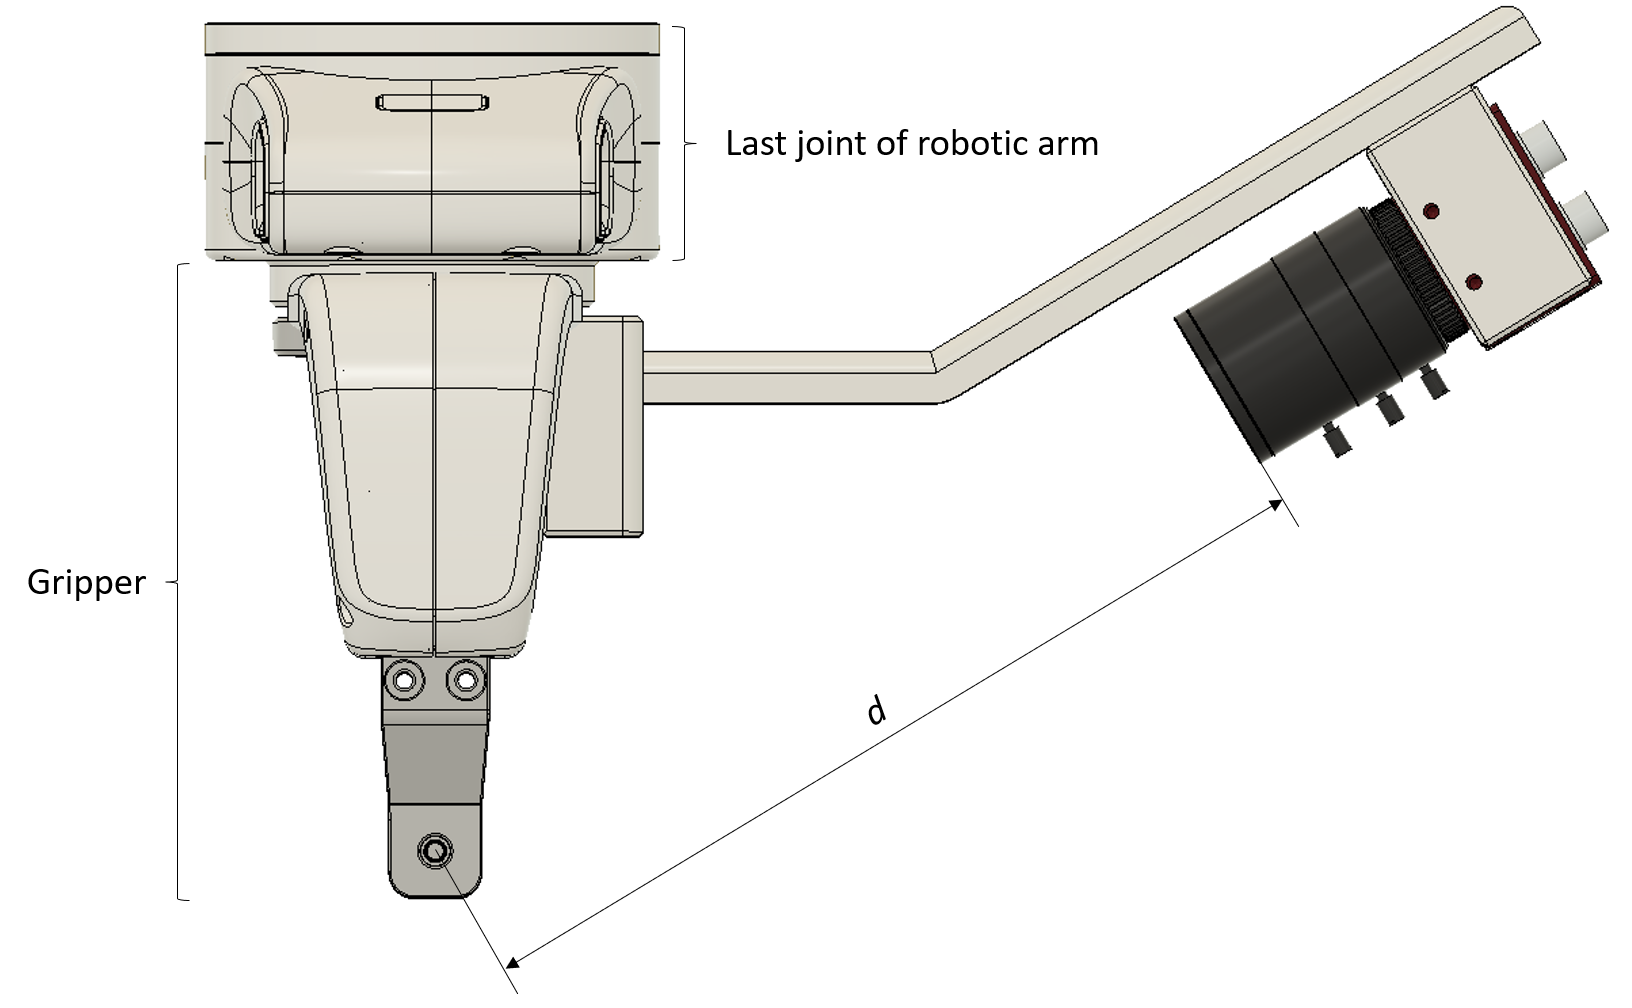
\includegraphics[width=\textwidth]{resources/images/assembly_description}
    \caption{Description of the assembly of the mount with the robotic arm, gripper and event-based camera.}\label{fig:assembly}
\end{figure}

In ~\Cref{fig:assembly} we can observe how all the components are assembled in CAD, and in ~\Cref{fig:assembly_real} the 3D printed mount, assembled with the robotic arm and the event-based camera, is shown.

\begin{figure}[H]
    \centering
    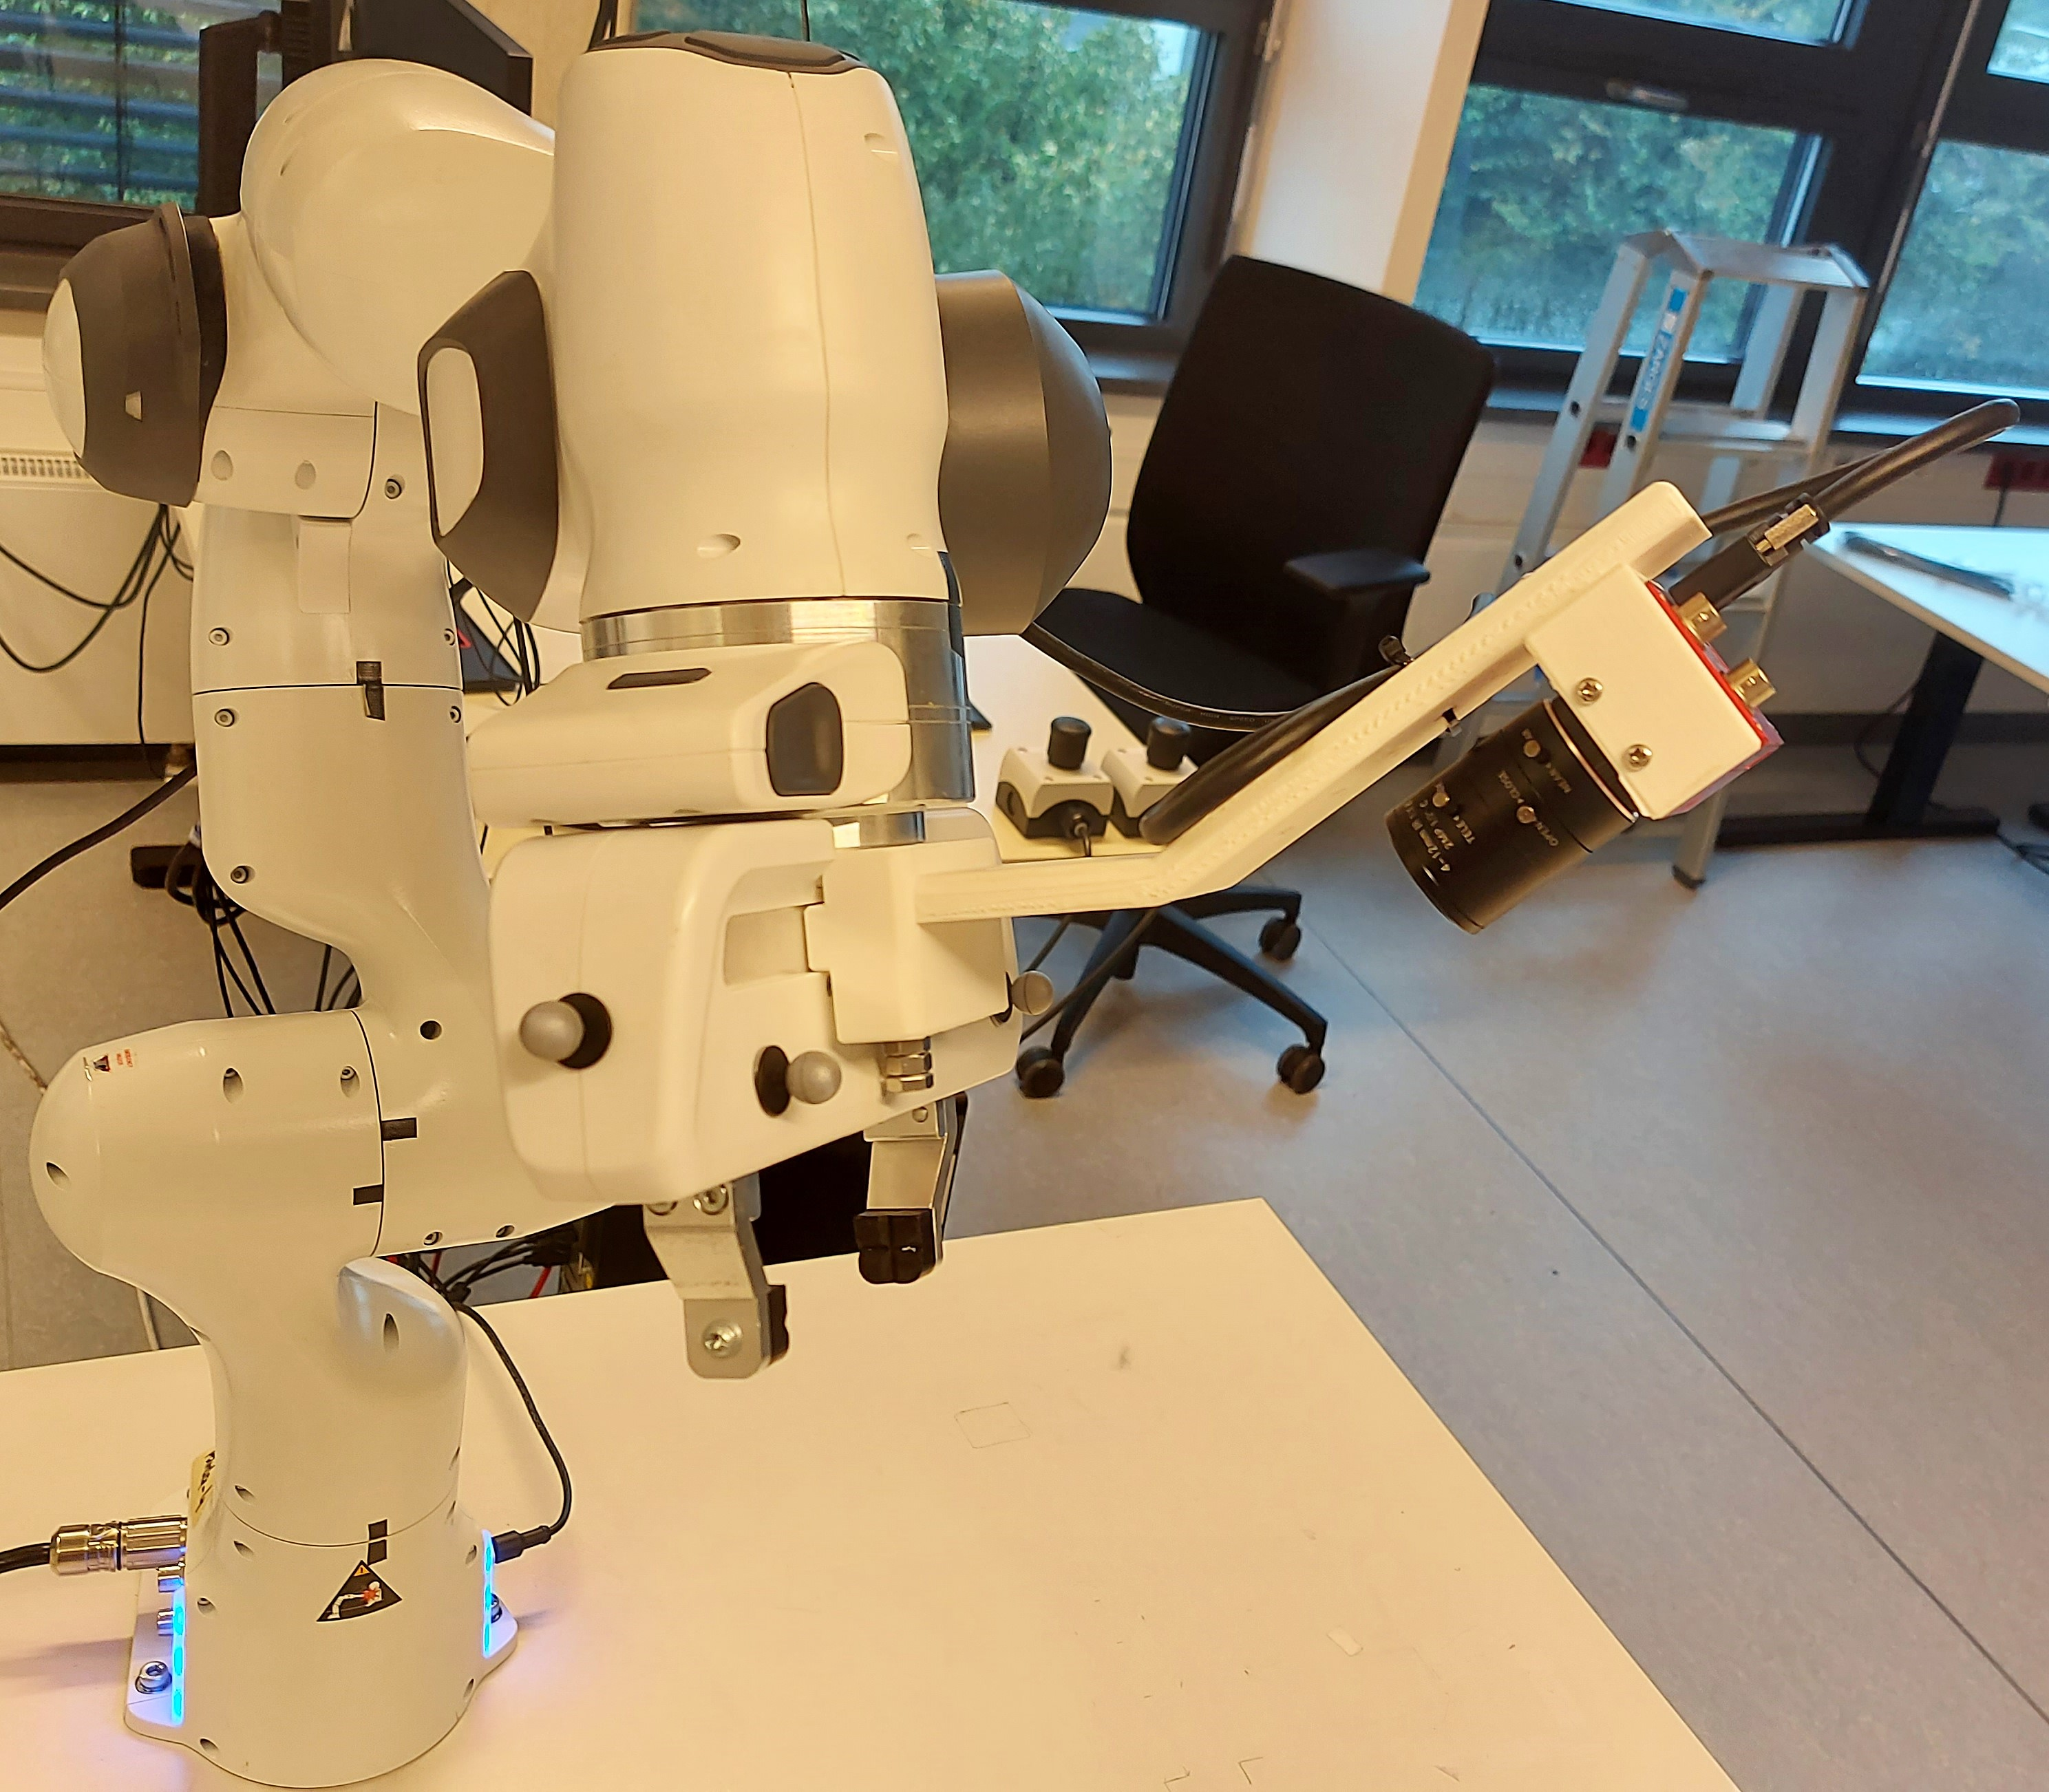
\includegraphics[width=0.85\textwidth]{resources/images/assembly_real}
    \caption{3D printed mount assembled with the robotic arm and event-based camera.}\label{fig:assembly_real}
\end{figure}

In addition, the camera can be connected to the mount using the spherical joint depicted in ~\Cref{fig:spherical}, using the holes provided in part A of the mount (see ~\Cref{fig:mount}). This joint enables the adjustment of not only the distance to the gripper, but also the orientation of the camera.

\begin{figure}[H]
    \centering
    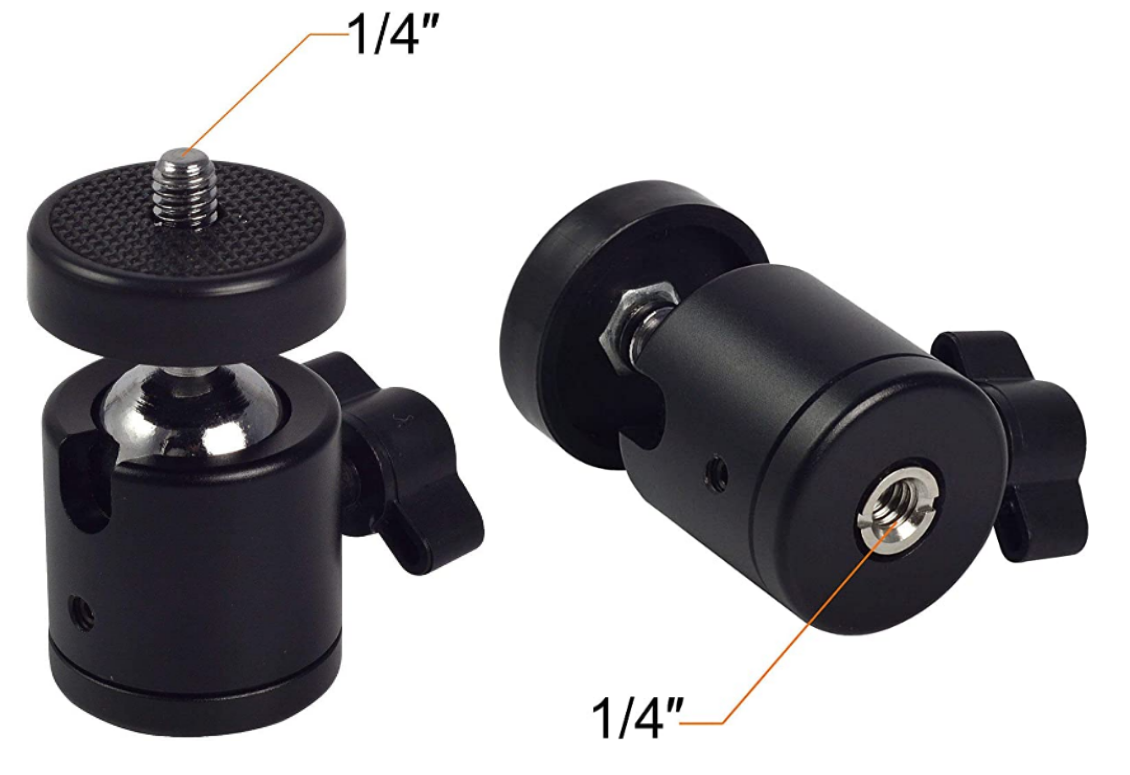
\includegraphics[width=0.6\textwidth]{resources/images/sphericaljoint}
    \caption{Spherical joint for cameras.}\label{fig:spherical}
\end{figure}

\section{Software}

\subsection{Required packages}

In order to control the robot arm and the gripper we use the \textit{botop}\footnote{\url{https://github.com/MarcToussaint/botop}} repository, which is used by the Learning \& Intelligent Systems (LIS) Lab at the TU Berlin.\\

To read and view the output provided by the camera DAVIS 346, we need the \textit{rpg\textunderscore dvs\textunderscore ros}\footnote{\url{https://github.com/uzh-rpg/rpg\textunderscore dvs\textunderscore ros}} package, which includes the C++ drivers and operates through Robot Operating System (ROS), a widely used framework for writing robot software.

\subsection{Developed code}

As the used setup and our needs differ from the ones of the LIS Lab, we needed to introduce some changes to the code and add some features to the existing \textit{botop} repository, creating a new repository\footnote{\url{https://github.com/MarcToussaint/co-ara/tree/ros_wrapper}} built on top of the aforementioned. Concretely, the trajectory was tuned, so that it was abrupt in the beginning to induce slip and ROS functionalities were added in order to be able to publish, and afterwards record, the information available inside the code.

\section{Calibration}

First, it is really important to configure the end-effector characteristics, as we are no longer using only the known two-finger gripper, but also the camera mount and the DAVIS 346. When configured incorrectly, gravitational forces are not entirely compensated and the robotic arm may pull towards certain directions in guiding mode, the regulation in operating mode may be affected so that the expected sensitivity of the arm for collision detection is reduced and the tracking behavior may be affected.\\

The new mass of the end-effector can be easily determined as the weight of all the elements (gripper, event-based camera and its mount with the screws) is known. However, the cable connected to the DAVIS 346 may introduce some slight changes. In terms of the center of mass and the inertia tensor, they were estimated using the CAD model of the elements (without considering the screws nor the cable) as a first estimation. Afterwards, using the command line tool \texttt{bot -float}, provided by the \textit{botop} repository, we could set the robot in a floating mode, where initially, if not configured properly, the robot tends to compensate the gravitational forces and move. So, by trial and error, the mass and center of mass were fine-tuned until the robot stayed still in the floating mode.\\

Also, to compute the trajectory, a collision checking is performed, however, the existing models in \textit{botop} repository are no longer valid, as the camera and its mount may collide with the table when grasping the object. Thus, the configuration file should be modified accordingly, resulting in the model shown in ~\Cref{fig:collision}. Finally, a frame is added to the camera lens, so that its pose and velocities are available.

\begin{figure}[H]
    \centering
    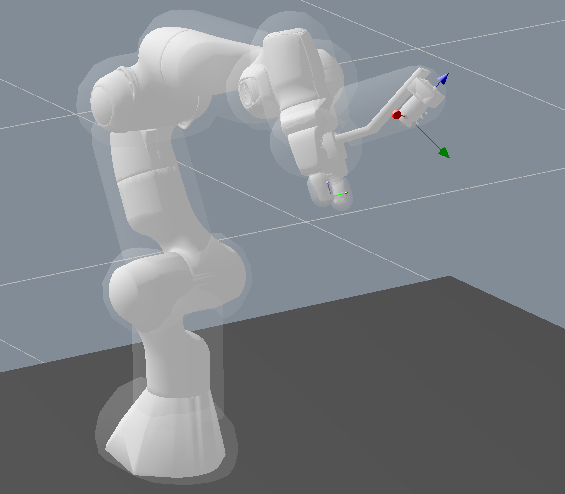
\includegraphics[width=0.7\textwidth]{resources/images/collision}
    \caption{Robot model including gripper with the camera and its mount.}\label{fig:collision}
\end{figure}

\section{Conclusion}

All in all, the described elements form the experiment setup, shown in ~\Cref{fig:setup}. As one may notice, the robot arm is placed above a white table, where the pick-and-place of the object is executed.

\begin{figure}[H]
    \centering
    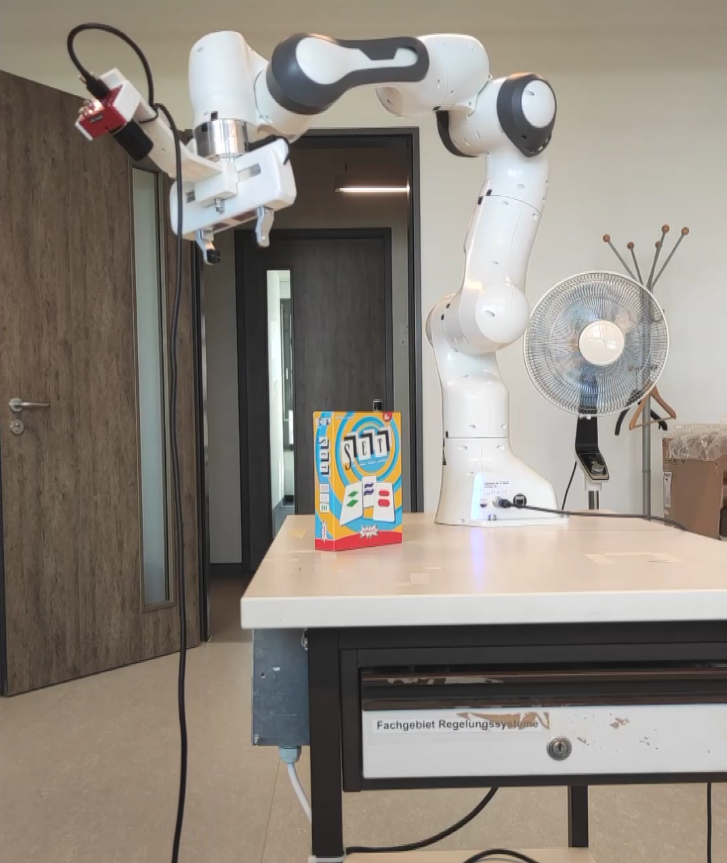
\includegraphics[width=0.8\textwidth]{resources/images/setup}
    \caption{Experiment setup: robotic arm, gripper, event-based camera and its mount.}\label{fig:setup}
\end{figure}

Using this setup, we were able to record data of slip and non-slip scenarios in different phases. After each recording phase, the data was analyzed, new requirements were noticed and new data was collected taking these into consideration. The results of the data collection are presented in the following chapter.
